\documentclass{article}
\usepackage[spanish]{babel}
\usepackage{graphicx}
\usepackage{subfigure}
\usepackage{listings}
\setlength{\parindent}{0pt}
\setlength{\parskip}{3mm}
\usepackage[numbers]{natbib}
\usepackage{color}
\definecolor{dkgreen}{rgb}{0,0.6,0}
\definecolor{gray}{rgb}{0.5,0.5,0.5}
\definecolor{mauve}{rgb}{0.58,0,0.82}
\usepackage{graphicx}
\usepackage{geometry}
\addtolength{\topmargin}{-.70in}
\addtolength{\textheight}{1in}
\usepackage{booktabs}
\usepackage[dvipsnames]{xcolor}

\usepackage{colortbl}
\lstset{ 
  backgroundcolor=\color{white},   % choose the background color; you must add \usepackage{color} or \usepackage{xcolor}; should come as last argument
  basicstyle=\footnotesize,        % the size of the fonts that are used for the code
  breakatwhitespace=false,         % sets if automatic breaks should only happen at whitespace
  breaklines=true,                 % sets automatic line breaking
  captionpos=b,                    % sets the caption-position to bottom
  commentstyle=\color{dkgreen},    % comment style
  deletekeywords={...},            % if you want to delete keywords from the given language
  escapeinside={\%}{)},          % if you want to add LaTeX within your code
  extendedchars=true,              % lets you use non-ASCII characters; for 8-bits encodings only, does not work with UTF-8
  firstnumber=1,                % start line enumeration with line 1000
  frame=single,	                   % adds a frame around the code
  keepspaces=true,                 % keeps spaces in text, useful for keeping indentation of code (possibly needs columns=flexible)
  keywordstyle=\color{blue},       % keyword style
  language=Octave,                 % the language of the code
  morekeywords={*,...},            % if you want to add more keywords to the set
  numbers=left,                    % where to put the line-numbers; possible values are (none, left, right)
  numbersep=5pt,                   % how far the line-numbers are from the code
  numberstyle=\tiny\color{gray}, % the style that is used for the line-numbers
  rulecolor=\color{black},         % if not set, the frame-color may be changed on line-breaks within not-black text (e.g. comments (green here))
  showspaces=false,                % show spaces everywhere adding particular underscores; it overrides 'showstringspaces'
  showstringspaces=false,          % underline spaces within strings only
  showtabs=false,                  % show tabs within strings adding particular underscores
  stepnumber=1,                    % the step between two line-numbers. If it's 1, each line will be numbered
  stringstyle=\color{mauve},     % string literal style
  tabsize=2,	                   % sets default tabsize to 2 spaces
  title=\lstname                  % show the filename of files included with \lstinputlisting; also try caption instead of title
}
\title{
Tarea 5
}
\author{5280}
\date{\today}
\begin{document}
\maketitle

\section*{Generador de grafos} 

En los grafos presentados, los nodos representan enrutadores en redes locales de comunicación. Se asume que la capacidad de los enlaces está determinada por el tipo de enlace físico que une los  enrutadores y no por las características de los mismos. 

Para la generación se emplea el algoritmo \texttt{dense\_gnm\_random}, que recibe como parámetros directamente el número de nodos y el número de aristas, lo que resulta cómodo para simular este tipo de redes.

\section*{Algoritmo de flujo máximo}

El algoritmo de flujo máximo elegido fue el Edmond Karp, pues fue el que mejores resultados mostró en la tarea anterior. Este algoritmo recibe como parámetros el grafo, el nodo fuente y el nodo sumidero.

\section*{Algoritmo de ordenamiento}

El algoritmo de ordenamiento empleado es el propuesto por Fruchterman y Reingold \citep{fruchterman1991graph}. Este muestra buenos resultados en la distribución de nodos, tamaño de las aristas uniforme y simetría de manera general, enfocándose en la velocidad y simplicidad.

\section*{Generación de grafos}

Para realizar el experimento son generados 5 grafos aleatoriamente, con la capacidad de flujo en sus aristas, distribuida normalmente, como puede observarse en la figura 1. El ancho de las aristas es proporcional a su capacidad. 

\begin{figure}[htbp]
\centering
\subfigure[Grafo 1]{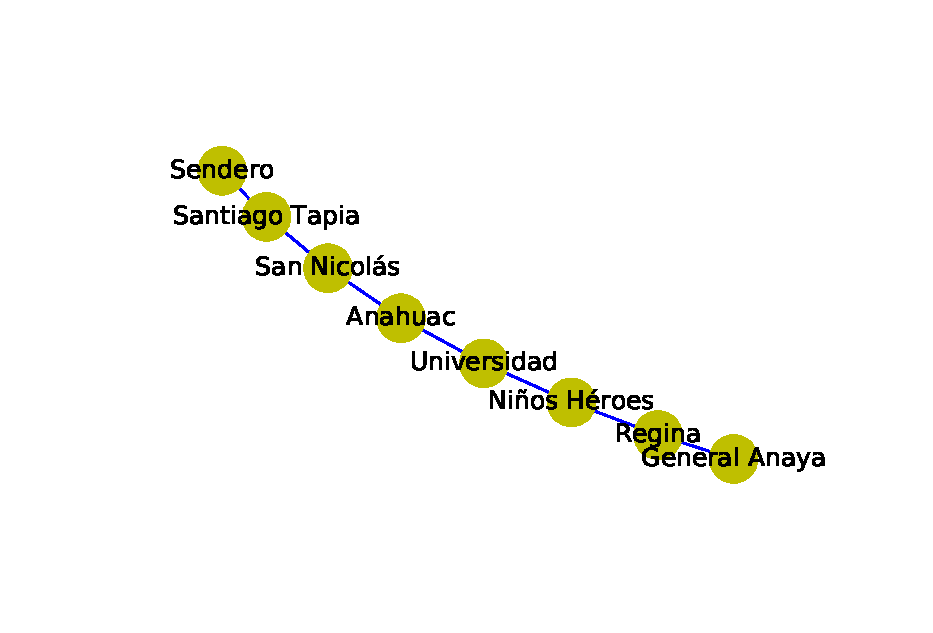
\includegraphics[scale=0.45]{fig1.eps}}
\subfigure[Grafo 2]{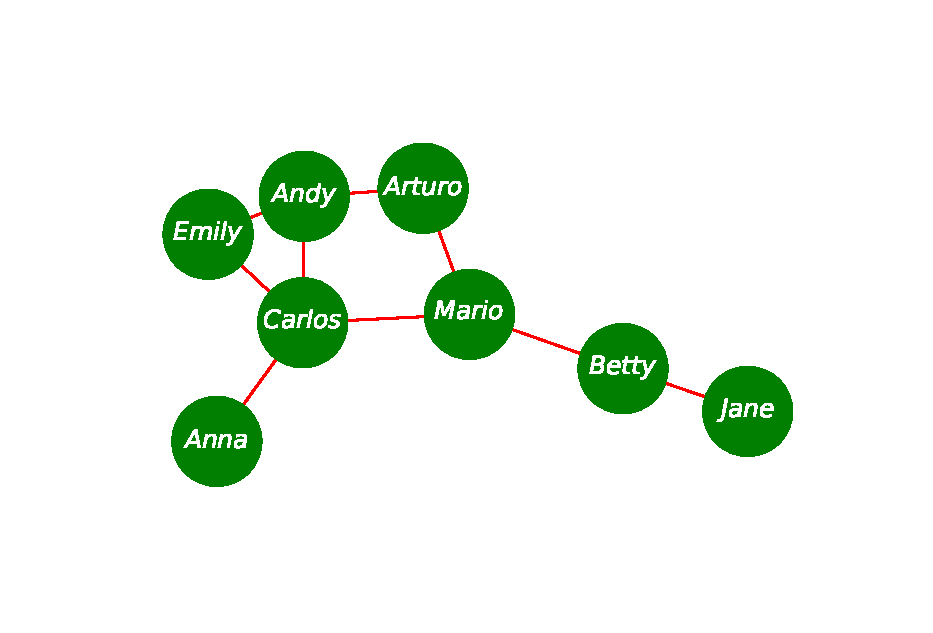
\includegraphics[scale=0.45]{fig2.eps}}
\subfigure[Grafo 3]{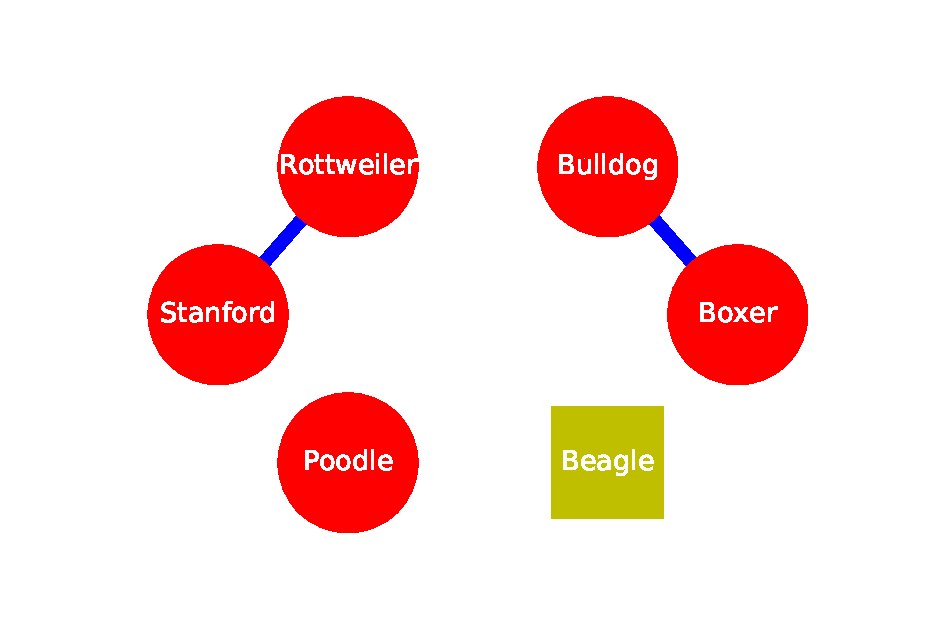
\includegraphics[scale=0.45]{fig3.eps}}
\subfigure[Grafo 4]{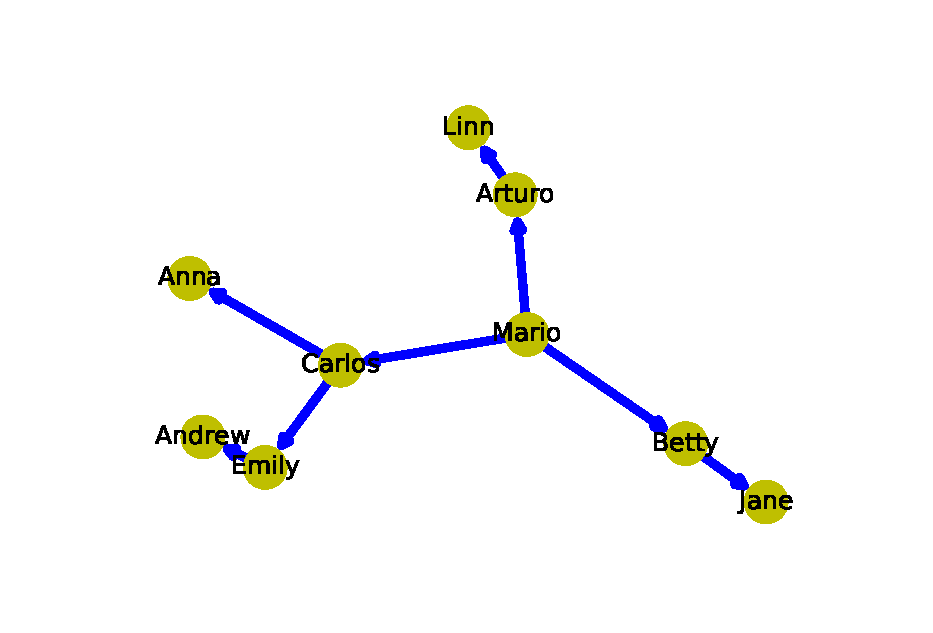
\includegraphics[scale=0.45]{fig4.eps}}
\subfigure[Grafo 5]{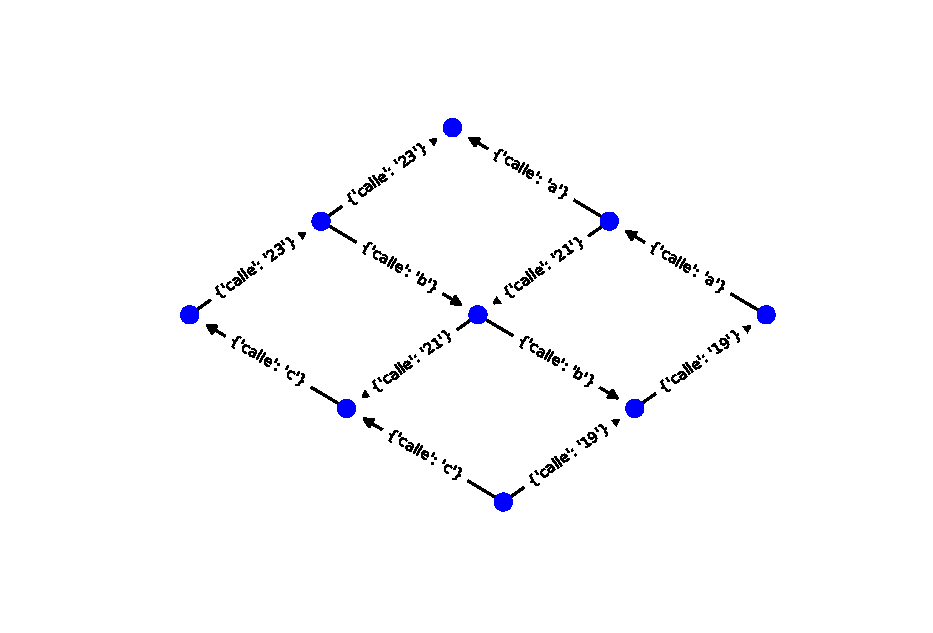
\includegraphics[scale=0.45]{fig5.eps}}
\caption{Grafos generados}
\label{Grafos} 
\end{figure}

\section*{Características estructurales de los nodos}
A cada uno de los grafos se les calculan las siguientes características estructurales de sus nodos:

\begin{itemize}
\item Distribución de grado (figura 2) 
\item Coeficiente de agrupamiento (figura 3) 
\item Centralidad de cercanía (figura 4)	
\item Centralidad de carga (figura 5) 
\item Excentricidad (figura 6)
\item Rango de página (figura 7) 	
\end{itemize}


\begin{figure}[htbp]
\subfigure[Grafo 1]{\includegraphics[scale=0.25]{Grado_grafo_0.eps}}
\subfigure[Grafo 2]{\includegraphics[scale=0.25]{CoefA_grafo_1.eps}}
\subfigure[Grafo 3]{\includegraphics[scale=0.25]{CoefA_grafo_2.eps}}
\subfigure[Grafo 4]{\includegraphics[scale=0.25]{CoefA_grafo_3.eps}}
\subfigure[Grafo 5]{\includegraphics[scale=0.25]{CoefA_grafo_4.eps}}
\caption{Histogramas de la distribución de grado para cada grafo}
\label{Grado} 
\end{figure}

\begin{figure}[htbp]
\subfigure[Grafo 1]{\includegraphics[scale=0.25]{Grado_grafo_0.eps}}
\subfigure[Grafo 2]{\includegraphics[scale=0.25]{Grado_grafo_1.eps}}
\subfigure[Grafo 3]{\includegraphics[scale=0.25]{Grado_grafo_2.eps}}
\subfigure[Grafo 4]{\includegraphics[scale=0.25]{Grado_grafo_3.eps}}
\subfigure[Grafo 5]{\includegraphics[scale=0.25]{Grado_grafo_4.eps}}
\caption{Histogramas del coeficiente de agrupamiento para cada grafo}
\label{CoefA} 
\end{figure}

\begin{figure}[htbp]
\subfigure[Grafo 1]{\includegraphics[scale=0.25]{CentCe_grafo_0.eps}}
\subfigure[Grafo 2]{\includegraphics[scale=0.25]{CentCe_grafo_1.eps}}
\subfigure[Grafo 3]{\includegraphics[scale=0.25]{CentCe_grafo_2.eps}}
\subfigure[Grafo 4]{\includegraphics[scale=0.25]{CentCe_grafo_3.eps}}
\subfigure[Grafo 5]{\includegraphics[scale=0.25]{CentCe_grafo_4.eps}}
\caption{Histogramas de la centralidad de cercanía para cada grafo}
\label{CentCe} 
\end{figure}

\begin{figure}[htbp]
\subfigure[Grafo 1]{\includegraphics[scale=0.25]{CentCa_grafo_0.eps}}
\subfigure[Grafo 2]{\includegraphics[scale=0.25]{CentCa_grafo_1.eps}}
\subfigure[Grafo 3]{\includegraphics[scale=0.25]{CentCa_grafo_2.eps}}
\subfigure[Grafo 4]{\includegraphics[scale=0.25]{CentCa_grafo_3.eps}}
\subfigure[Grafo 5]{\includegraphics[scale=0.25]{CentCa_grafo_4.eps}}
\caption{Histogramas de la centralidad de carga para cada grafo}
\label{CentCa} 
\end{figure}

\begin{figure}[htbp]
\subfigure[Grafo 1]{\includegraphics[scale=0.24]{Excent_grafo_0.eps}}
\subfigure[Grafo 2]{\includegraphics[scale=0.24]{Excent_grafo_1.eps}}
\subfigure[Grafo 3]{\includegraphics[scale=0.24]{Excent_grafo_2.eps}}
\subfigure[Grafo 4]{\includegraphics[scale=0.24]{Excent_grafo_3.eps}}
\subfigure[Grafo 5]{\includegraphics[scale=0.24]{Excent_grafo_4.eps}}
\caption{Histogramas de la excentricidad para cada grafo}
\label{Excent} 
\end{figure}

\begin{figure}[htbp]
\subfigure[Grafo 1]{\includegraphics[scale=0.25]{PageR_grafo_0.eps}}
\subfigure[Grafo 2]{\includegraphics[scale=0.25]{PageR_grafo_1.eps}}
\subfigure[Grafo 3]{\includegraphics[scale=0.25]{PageR_grafo_2.eps}}
\subfigure[Grafo 4]{\includegraphics[scale=0.25]{PageR_grafo_3.eps}}
\subfigure[Grafo 5]{\includegraphics[scale=0.25]{PageR_grafo_4.eps}}
\caption{Histogramas de la excentricidad para cada grafo}
\label{PageR} 
\end{figure}

\section*{Flujo máximo}

Para cada combinación de fuente-sumidero en cada grafo se calcula el flujo máximo. En las figuras 8, 9, 10, 11 y 12, se visualizan los flujos para la mejor y peor pareja de fuente-sumidero para los grafos 1, 2, 3, 4 y 5, respectivamente. Los nodos rojos representan las mejores fuente-sumidero, como los grafos son no dirigidos, estos son intercambiables. Los nodos azules son buenas fuente-sumidero y los nodos grises son las peores fuentes-sumideros, en cada grafo. 

En rosado se muestra cuanto flujo pasa por cada arista una vez aplicado al algoritmo de flujo máximo, aunmentando la intensidad del color proporcionalmente a la cantidad de flujo. En las aristas negras no pasa flujo.

\begin{figure}[htbp]
\subfigure[Mejor pareja, flujo: 73]{\includegraphics[scale=0.55]{mejor1.eps}}
\subfigure[Peor pareja, flujo: 11]{\includegraphics[scale=0.55]{peor1.eps}}
\caption{Visualización de la mejor y peor pareja de nodos a usar como fuente o sumidero en el grafo 1}
\label{Flujo1} 
\end{figure}

\begin{figure}[htbp]
\subfigure[Mejor pareja, flujo: 66]{\includegraphics[scale=0.55]{mejor2.eps}}
\subfigure[Peor pareja, flujo: 9]{\includegraphics[scale=0.55]{peor2.eps}}
\caption{Visualización de la mejor y peor pareja de nodos a usar como fuente o sumidero en el grafo 2}
\label{Flujo2} 
\end{figure}

\begin{figure}[htbp]
\subfigure[Mejor pareja, flujo: 59]{\includegraphics[scale=0.55]{mejor3.eps}}
\subfigure[Peor pareja, flujo: 19]{\includegraphics[scale=0.55]{peor3.eps}}
\caption{Visualización de la mejor y peor pareja de nodos a usar como fuente o sumidero en el grafo 3}
\label{Flujo3} 
\end{figure}

\begin{figure}[htbp]
\subfigure[Mejor pareja, flujo: 66]{\includegraphics[scale=0.55]{mejor4.eps}}
\subfigure[Peor pareja, flujo: 11]{\includegraphics[scale=0.55]{peor4.eps}}
\caption{Visualización de la mejor y peor pareja de nodos a usar como fuente o sumidero en el grafo 4}
\label{Flujo4} 
\end{figure}


\begin{figure}[htbp]
\subfigure[Mejor pareja, flujo: 59]{\includegraphics[scale=0.55]{mejor5.eps}}
\subfigure[Peor pareja, flujo: 21]{\includegraphics[scale=0.55]{peor5.eps}}
\caption{Visualización de la mejor y peor pareja de nodos a usar como fuente o sumidero en el grafo 5.}
\label{Flujo5} 
\end{figure}

\section*{Influencia de las características estructurales del grafo en el tiempo de ejecución}


En el Cuadro 1 se muestran los resultados del análisis de varianza (ANOVA en lo adelante, por sus siglas en inglés) de las carácterísticas estructurales del grafo para ver su influencia en el tiempo de ejecución del algoritmo de flujo máximo.

Se aprecia que las carácterísticas estructurales de los grafos no influyen en el tiempo de ejecución del alogoritmo de flujo máximo para los grafos generados. 
Se observa, además, que existe una relación entre las siguientes características:


\begin{itemize}
\item Distribución de grado y coeficiente de agrupamiento 
\item Distribución de grado y centralidad de cercanía
\item Distribución de grado y centralidad de carga
\item Rango de página y centralidad de cercanía
\item Rango de página y centralidad de carga
\end{itemize}

\newpage

% Table generated by Excel2LaTeX from sheet 'modelo'
\begin{table}
  \centering
  \caption{Resultado del ANOVA para los valores de tiempo}
    \begin{tabular}{|l|r|r|r|r|}
    \toprule
    \rowcolor[rgb]{ .357,  .608,  .835} \textbf{Factor} & \multicolumn{1}{l|}{\textbf{suma\_cuad}} & \multicolumn{1}{l|}{\textbf{Grados de libertad}} & \multicolumn{1}{l|}{\textbf{F}} & \multicolumn{1}{l|}{\textbf{Prueba}} \\
    \midrule
    Grado & 8.12E-08 & 1     & 0.96  & 0.33 \\
    \midrule
    CoefA & 6.78E-08 & 1     & 0.8   & 0.37 \\
    \midrule
    CentCe & 5.12E-09 & 1     & 0.06  & 0.8 \\
    \midrule
    CentCa & 2.16E-07 & 1     & 2.5   & 0.11 \\
    \midrule
    Excent & 2.32E-08 & 1     & 0.27  & 0.6 \\
    \midrule
    RangoP & 2.11E-07 & 1     & 2.48  & 0.11 \\
    \midrule
    Grado:CoefA & 4.45E-07 & 1     & 5.23  & 0.02 \\
    \midrule
    Grado:CentCe & 1.00E-06 & 1     & 11.8  & 0.0006 \\
    \midrule
    Grado:CentCa & 1.55E-06 & 1     & 18.28 & 2.00E-05 \\
    \midrule
    Grado:Excent & 1.84E-07 & 1     & 2.16  & 0.14 \\
    \midrule
    Grado:RangoP & 2.30E-07 & 1     & 2.7   & 0.1 \\
    \midrule
    CentCe:CentCa & 2.11E-07 & 1     & 2.48  & 0.12 \\
    \midrule
    CentCe:Excent & 1.53E-07 & 1     & 1.8   & 0.18 \\
    \midrule
    CentCe:RangoP & 7.70E-07 & 1     & 9.06  & 0.002 \\
    \midrule
    CentCa:Excent & 1.30E-07 & 1     & 1.53  & 0.22 \\
    \midrule
    CentCa:RangoP & 1.89E-06 & 1     & 22.25 & 2.50E-06 \\
    \midrule
    Excent:RangoP & 1.52E-07 & 1     & 1.79  & 0.18 \\
    \midrule
    Residual & 0.00015678 & 1844  &       &  \\
    \bottomrule
    \end{tabular}%
  \label{tab:Cuadro 1}%
\end{table}%

\section*{Influecia de las características estructurales del grafo en el flujo máximo}

En el Cuadro 1 se muestra el ANOVA de las carácterísticas estructurales del grafo para analizar su influencia en el flujo máximo.

Se aprecia inciden en el flujo máximo las siguientes características estructurales:  

\begin{itemize}
\item Coeficiente de agrupamiento 
\item Centralidad de carga
\item Rango de página 
\end{itemize}

Se observa, además, que existe una relación entre las siguientes características:

\begin{itemize}
\item Distribución de grado y coeficiente de agrupamiento 
\item Distribución de grado y rango de página
\item Coeficiente de agrupamiento y centralidad de cercanía
\item Coeficiente de agrupamiento y rango de página

\end{itemize}

% Table generated by Excel2LaTeX from sheet 'modeloFlujomaximo'
\begin{table}[htbp]
  \centering
  \caption{Resultado del ANOVA para los valores de flujo máximo}
    \begin{tabular}{|l|r|r|r|r|}
    \toprule
    \rowcolor[rgb]{ .357,  .608,  .835} \textbf{Factor} & \multicolumn{1}{l|}{\textbf{sum\_cuad}} & \multicolumn{1}{l|}{\textbf{Grados de libertad}} & \multicolumn{1}{l|}{\textbf{F}} & \multicolumn{1}{l|}{\textbf{Prueba}} \\
    \midrule
    Grado & 38.7288463 & 1     & 0.459047 & 0.498155 \\
    \midrule
    CoefA & 1363.23246 & 1     & 16.15817 & 6.06E-05 \\
    \midrule
    CentCe & 143.623743 & 1     & 1.702349 & 0.192144 \\
    \midrule
    CentCa & 976.245999 & 1     & 11.57129 & 0.000684 \\
    \midrule
    Excent & 155.426353 & 1     & 1.842243 & 0.174855 \\
    \midrule
    PageR & 508.236449 & 1     & 6.024044 & 0.014204 \\
    \midrule
    Grado:CoefA & 650.232041 & 1     & 7.707095 & 0.005556 \\
    \midrule
    Grado:CentCe & 93.006395 & 1     & 1.10239 & 0.29388 \\
    \midrule
    Grado:CentCa & 112.234812 & 1     & 1.330301 & 0.248901 \\
    \midrule
    Grado:Excent & 162.655867 & 1     & 1.927934 & 0.165153 \\
    \midrule
    Grado:PageR & 660.247786 & 1     & 7.82581 & 0.005204 \\
    \midrule
    CoefA:CentCe & 335.675561 & 1     & 3.978708 & 0.046226 \\
    \midrule
    CoefA:CentCa & 49.9598544 & 1     & 0.592166 & 0.441682 \\
    \midrule
    CoefA:Excent & 16.9158218 & 1     & 0.2005 & 0.65437 \\
    \midrule
    CoefA:PageR & 553.464369 & 1     & 6.560123 & 0.010508 \\
    \midrule
    CentCe:CentCa & 7.00601142 & 1     & 0.083041 & 0.77325 \\
    \midrule
    CentCe:Excent & 23.2094891 & 1     & 0.275098 & 0.599995 \\
    \midrule
    CentCe:PageR & 85.7199062 & 1     & 1.016024 & 0.313596 \\
    \midrule
    CentCa:Excent & 66.437239 & 1     & 0.78747 & 0.374982 \\
    \midrule
    CentCa:PageR & 106.077006 & 1     & 1.257314 & 0.262307 \\
    \midrule
    Excent:PageR & 104.744206 & 1     & 1.241516 & 0.265325 \\
    \midrule
    Residual & 155237.086 & 1840  &       &  \\
    \bottomrule
    \end{tabular}%
  \label{tab:Cuadro 2}%
\end{table}%

\section*{Código fuente utilizado para realizar el experimento}

\subsection*{Generación de grafos}

\lstinputlisting[language=Python, firstline=7,lastline=41]{Grafos.py} 

\subsection*{Cálculo de atributos}
\lstinputlisting[language=Python, firstline=117,lastline=129]{Programa.py} 

\subsection*{Cálculo de tiempo de ejecución y flujo máximo}
\lstinputlisting[language=Python, firstline=131,lastline=147]{Programa.py}


\subsection*{ANOVA}
\lstinputlisting[language=Python, firstline=22,lastline=26]{procesamiento.py}

\newpage
\bibliography{Tarea5}
\bibliographystyle{plain}
\end{document}